\documentclass[spanish]{beamer}
\usepackage[utf8]{inputenc}
\usepackage{float}
\usepackage{beamerthemesplit}
\usepackage{latexsym}
\usepackage[T1]{fontenc}
\usepackage{amsmath}
\usepackage{hyperref}
\usepackage{graphicx}
\usepackage{babel,blindtext}
\usepackage{amsfonts}
\usepackage[round]{natbib}
\bibliographystyle{chicago}
\usepackage{subcaption} 


\decimalpoint

\usetheme{Antibes}%este es el templete que se usa a lo largo de la presentacion
%themes
%   default
%   Boadilla
%   Madrid
%   Pittsburgh
%   Copenhagen
%   Warsaw
%   Singapore
%   Malmoe
\newcommand\Fontvi{\fontsize{6}{7.2}\selectfont}
\mode<presentation>%tipo de 
\begin{document}

%%%%%%%%%%%%%%%%%%%%%%%%%%%%%%%%%%%%%%%%%%%%%%%%%%%%%%%%%%%%%%%%%%%%%%%%%%%%%%%%%%%%%%%%%%%%%%%%%%%%%%%%%%%%%
\title{Descripción de datos con medidas numéricas}
\subtitle{Estadística}
\author{Gamaliel Moreno Chávez}
\institute{Centro de Crecimiento Humanista}
\date{Enero\\ 2021}%para que ponga la fecha de hoy 

\frame{\titlepage}
%%%%%%%%%%%%%%%%%%%%%%%%%%%%%%%%%%%%%%%%%%%%%%%%%%%%%%%%%%%%%%%%%%%%%%%%%%%%%%%%%%%%%%%%%%%%%%%%%%%%%%%%%%%%%
%%%%%%%%%%%%%%%%%%%%%%%%%%%%%%%%%%%%%%%%%%%%%%%%%%%%%%%%%%%%%%%%%%%%%%%%%%%%%%%%%%%%%%%%%%%%%%%%%%%%%%%%%%%%%%%%%%%%%%%%%%%%%%%%%%%%%%%%%%%%%%%%%%%%%%%%%%%%%%%%%%%%%%%%%%%%%%%%%%%%%%%%%%%%%%%%%%%%%%%%%%%%%%%%%%%%%%%%%%
%%%%%%%%%%%%%%%%%%%%%%%%%%%%%%%%%%%%%%%%%%%%%%%%%%%%%%%%%%%%%%%%%%%%%%%%%%%%%%%%%%%%%%%%%%%%%%%%%%%%%%%%%%%%%%%%%%%%%%%%%%%%%%%%%%%%%%%%%%%%%%%%%%%%%%%%%%%%%%%%%%%%%%%%%%%%%%%%%%%%%%%%%%%%%%%%%%%%%%%%%%%%%%%%%%%%%%%%%%

\begin{frame}
\frametitle{Generalidades}
Las gráficas pueden ayudar a describir la forma básica de una distribución de datos pero hay limitaciones
\begin{itemize}
\item No siempre es posible presentar gráficas.
\item Son poco precisas.
\item No son comparables
\end{itemize}
Una forma de superar estos problemas es usar medidas numéricas, que se pueden calcular para una muestra o una población de mediciones.
\end{frame}

%%%%%%%%%%%%%%%%%%%%%%%%%%%%%%%%%%%%%%%%%%%%%%%%%%%%%%%%%%%%%%%%%%%%%%%%%%%%%%%%%%%%%%%%%%%%%%%%%%%%%%%%%%%%%
\begin{frame}
\frametitle{Generalidades} 
Aplicaciones 
\begin{center}
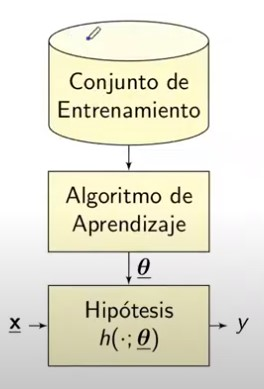
\includegraphics[scale=0.4]{im2}
\end{center}
\end{frame}
%%%%%%%%%%%%%%%%%%%%%%%%%%%%%%%%%%%%%%%%%%%%%%%%%%%%%%%%%%%%%%%%%%%%%%%%%%%%%%%%%%%%%%%%%%%%%%%%%%%%%%%%%%%%%
\begin{frame}
\frametitle{Generalidades} 
Aplicaciones 

\begin{center}
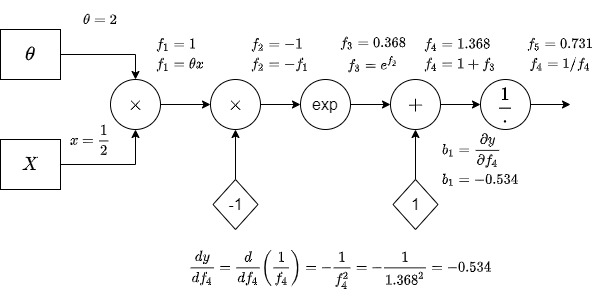
\includegraphics[scale=2]{im3}
\end{center}
\end{frame}
%%%%%%%%%%%%%%%%%%%%%%%%%%%%%%%%%%%%%%%%%%%%%%%%%%%%%%%%%%%%%%%%%%%%%%%%%%%%%%%%%%%%%%%%%%%%%%%%%%%%%%%%%%%%%
\begin{frame}
\frametitle{Generalidades} 
Aplicaciones 
\begin{center}
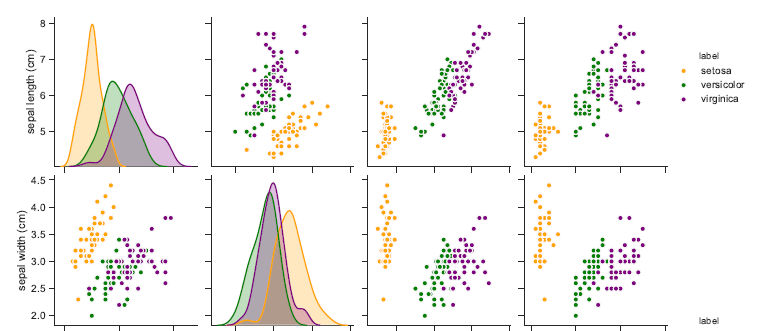
\includegraphics[scale=2]{im4}
\end{center}
\end{frame}
%%%%%%%%%%%%%%%%%%%%%%%%%%%%%%%%%%%%%%%%%%%%%%%%%%%%%%%%%%%%%%%%%%%%%%%%%%%%%%%%%%%%%%%%%%%%%%%%%%%%%%%%%%%%%
\begin{frame}
\frametitle{Generalidades} 
Aplicaciones 
\begin{center}
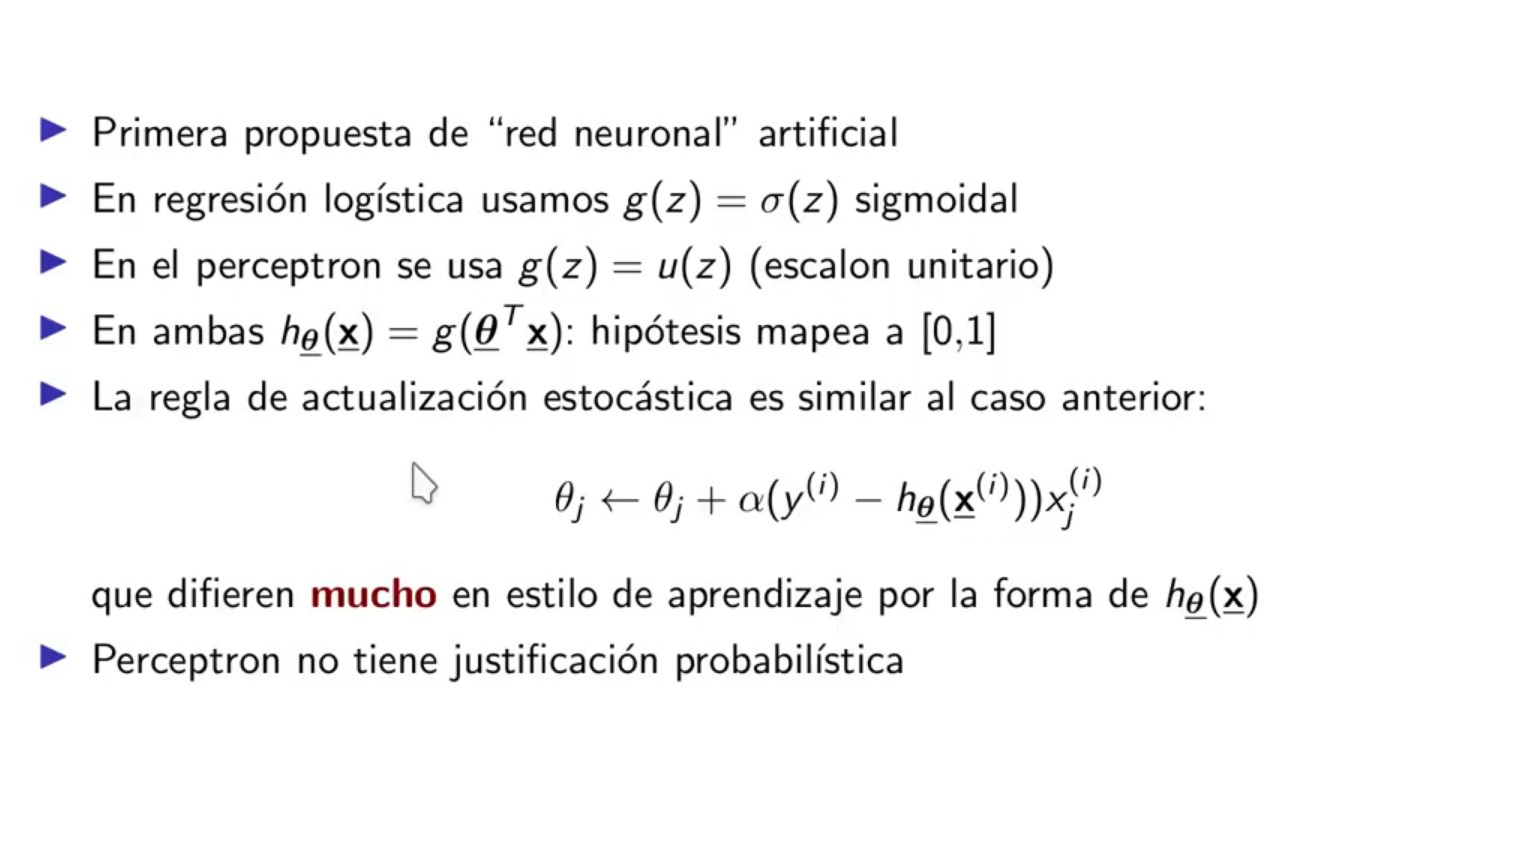
\includegraphics[scale=0.25]{im5}
\end{center}
\end{frame}

%%%%%%%%%%%%%%%%%%%%%%%%%%%%%%%%%%%%%%%%%%%%%%%%%%%%%%%%%%%%%%%%%%%%%%%%%%%%%%%%%%%%%%%%%%%%%%%%%%%%%%%%%%%%%
\begin{frame}
\frametitle{Introducción}

La Estadística resuelve problemas de 
\begin{block}{Análisis de muestras}
Se elige una muestra de una población para hacer inferencias respecto a esa población a partir de lo observado en la muestra (sondeos de opinión, control de calidad, etc).
\end{block}

\end{frame}
%%%%%%%%%%%%%%%%%%%%%%%%%%%%%%%%%%%%%%%%%%%%%%%%%%%%%%%%%%%%%%%%%%%%%%%%%%%%%%%%%%%%%%%%%%%%%%%%%%%%%%%%%%%%%
\begin{frame}
\frametitle{Introducción}
La Estadística resuelve problemas de 
\begin{block}{Descripción de datos}
Procedimientos para resumir la información contenida en un conjunto (amplio) de datos.
\end{block}

\end{frame}
%%%%%%%%%%%%%%%%%%%%%%%%%%%%%%%%%%%%%%%%%%%%%%%%%%%%%%%%%%%%%%%%%%%%%%%%%%%%%%%%%%%%%%%%%%%%%%%%%%%%%%%%%%%%%
\begin{frame}
\frametitle{Introducción}

La Estadística resuelve problemas de 
\begin{block}{Contraste de hipótesis}
Metodología estadística para diseñar experimentos que garanticen que las conclusiones que se extraigan sean válidas. Sirve para comparar las predicciones resultantes de las hipótesis con los datos observados (medicina eficaz, diferencias entre poblaciones, etc).
\end{block}

\end{frame}
%%%%%%%%%%%%%%%%%%%%%%%%%%%%%%%%%%%%%%%%%%%%%%%%%%%%%%%%%%%%%%%%%%%%%%%%%%%%%%%%%%%%%%%%%%%%%%%%%%%%%%%%%%%%%
\begin{frame}
\frametitle{Introducción}

La Estadística resuelve problemas de 
\begin{block}{Medición de relaciones}
Medición de relaciones entre variables estadísticas (contenido de gas hidrógeno neutro en galaxias y la
tasa de formación de estrellas, etc)
\end{block}
\begin{block}{Predicción}
Prever la evolución de una variable estudiando su historia y/o relación con otras variables.
\end{block}


\end{frame}
%%%%%%%%%%%%%%%%%%%%%%%%%%%%%%%%%%%%%%%%%%%%%%%%%%%%%%%%%%%%%%%%%%%%%%%%%%%%%%%%%%%%%%%%%%%%%%%%%%%%%%%%%%%%%
\begin{frame}
\frametitle{Introducción}
\begin{columns}
\column{0.5\textwidth}
\begin{block}{Estadística Descriptiva}
La cual es la que se utiliza en la descripción y análisis de conjuntos de datos o población.
\end{block}

\column{0.5\textwidth}
\begin{block}{Inferencia Estadística}
La cual hace posible la estimación de una característica de una población, o la toma de una decisión con respecto a una población, con base únicamente en resultados muestrales.
\end{block}

\end{columns}
\end{frame}
%%%%%%%%%%%%%%%%%%%%%%%%%%%%%%%%%%%%%%%%%%%%%%%%%%%%%%%%%%%%%%%%%%%%%%%%%%%%%%%%%%%%%%%%%%%%%%%%%%%%%%%%%%%%%
\begin{frame}
\frametitle{Universo}
Población o Universo: Conjunto completo de individuos, objetos, o medidas los cuales poseen
una característica común observable y que serán considerados en un estudio.
\begin{columns}
\column{0.5\textwidth}
\begin{center}
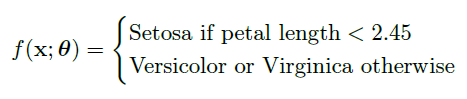
\includegraphics[scale=0.6]{im6}
\end{center}

\column{0.5\textwidth}
Con información obtenida de una muestra representativa de
esa población, tratamos de describir o pronosticar el comportamiento de la población.
\end{columns}
\end{frame}
%%%%%%%%%%%%%%%%%%%%%%%%%%%%%%%%%%%%%%%%%%%%%%%%%%%%%%%%%%%%%%%%%%%%%%%%%%%%%%%%%%%%%%%%%%%%%%%%%%%%%%%%%%%%%
\begin{frame}
\frametitle{Parámetros}
Caracteres cuantitativos o cualitativos. El objeto de nuestra medida pueden ser caracteres de tipos muy diversos. De ahí que normalmente se clasifiquen en:
\begin{itemize}
\item \textbf{Cuantitativos}: aquellos que toman valores numéricos
\item \textbf{Cualitativos}: también llamados atributos, son aquellos que no podemos representar numéricamente y describen cualidades.
\end{itemize}

\end{frame}
%%%%%%%%%%%%%%%%%%%%%%%%%%%%%%%%%%%%%%%%%%%%%%%%%%%%%%%%%%%%%%%%%%%%%%%%%%%%%%%%%%%%%%%%%%%%%%%%%%%%%%%%%%%%%
\begin{frame}
\frametitle{Variable Aleatoria}
Una \textbf{variable} es una característica que cambia o varía con el tiempo y/o para diferentes personas u objetos bajo consideración.
\begin{itemize}
\item \textbf{Variables Cualitativas}: son aquellas que pueden expresarse sólo en forma de atributo.
\item \textbf{Variables Cuantitativas}: son aquellas variables que pueden expresarse en forma numérica. Se
dividen en discretas y continuas.
\end{itemize}

\end{frame}
%%%%%%%%%%%%%%%%%%%%%%%%%%%%%%%%%%%%%%%%%%%%%%%%%%%%%%%%%%%%%%%%%%%%%%%%%%%%%%%%%%%%%%%%%%%%%%%%%%%%%%%%%%%%%
\begin{frame}
\frametitle{Variable Aleatoria}
Ejemplos de Variables cualitativas
\vspace{1em}
\begin{columns}
\column{0.5\textwidth}
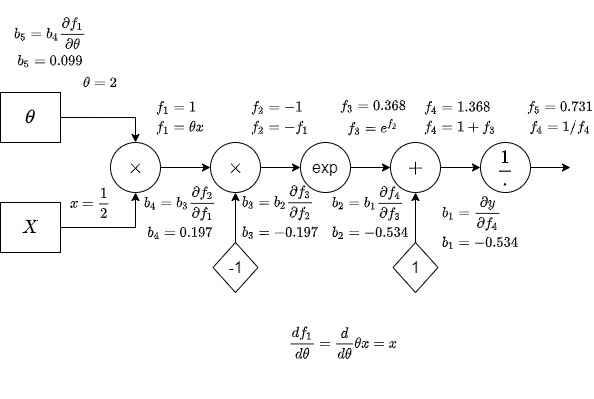
\includegraphics[scale=0.5]{im7}

\column{0.5\textwidth}
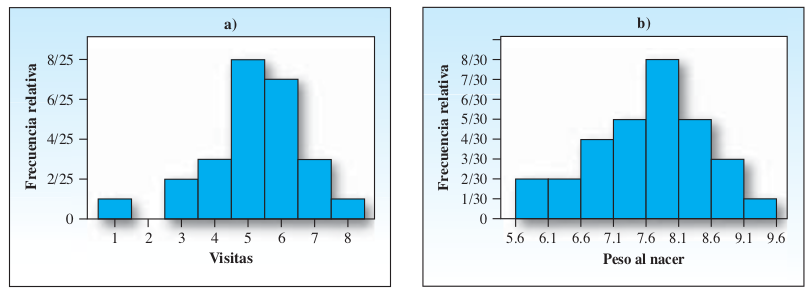
\includegraphics[scale=0.5]{im8}

\end{columns}
\end{frame}
%%%%%%%%%%%%%%%%%%%%%%%%%%%%%%%%%%%%%%%%%%%%%%%%%%%%%%%%%%%%%%%%%%%%%%%%%%%%%%%%%%%%%%%%%%%%%%%%%%%%%%%%%%%%%
\begin{frame}
\frametitle{Variable Aleatoria}
\textbf{Variables Cuantitativas Discretas}, son respuestas numéricas que surgen de un proceso de conteo, siendo siempre un número entero.\vspace{1em}

1) Número de asignaturas inscritas en el semestre.

2) Número de integrantes del grupo familiar.

3) Número de salas de clases.

\end{frame}
%%%%%%%%%%%%%%%%%%%%%%%%%%%%%%%%%%%%%%%%%%%%%%%%%%%%%%%%%%%%%%%%%%%%%%%%%%%%%%%%%%%%%%%%%%%%%%%%%%%%%%%%%%%%%
\begin{frame}
\frametitle{Variable Aleatoria}
\textbf{Variables Cuantitativas Continuas}, son respuestas numéricas que surgen de un proceso de medición, las cuales pueden tomar valores entre dos números enteros.\vspace{1em}

1) Estatura

2) Temperatura

3) Peso

\end{frame}
%%%%%%%%%%%%%%%%%%%%%%%%%%%%%%%%%%%%%%%%%%%%%%%%%%%%%%%%%%%%%%%%%%%%%%%%%%%%%%%%%%%%%%%%%%%%%%%%%%%%%%%%%%%%%
\begin{frame}
\frametitle{Variable Aleatoria}
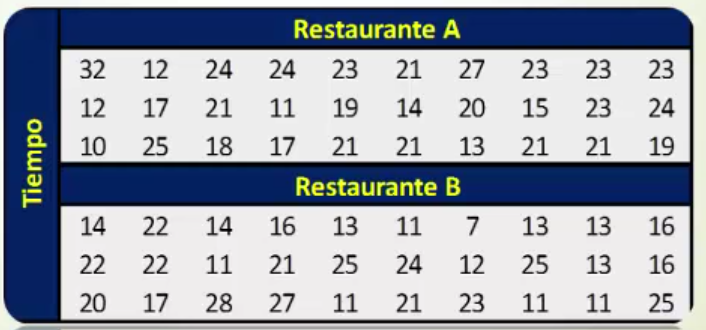
\includegraphics[scale=0.4]{im9}

\end{frame}
%%%%%%%%%%%%%%%%%%%%%%%%%%%%%%%%%%%%%%%%%%%%%%%%%%%%%%%%%%%%%%%%%%%%%%%%%%%%%%%%%%%%%%%%%%%%%%%%%%%%%%%%%%%%%
\begin{frame}
\frametitle{Gráficas para datos}
Una vez recolectados los datos, éstos pueden consolidarse y resumirse para mostrar la siguiente información:
\vspace{1em}

• La \textbf{frecuencia} o número de mediciones en cada categoría

• La \textbf{frecuencia relativa} o proporción de mediciones en cada categoría

• El \textbf{porcentaje} de mediciones en cada categoría
\end{frame}

%%%%%%%%%%%%%%%%%%%%%%%%%%%%%%%%%%%%%%%%%%%%%%%%%%%%%%%%%%%%%%%%%%%%%%%%%%%%%%%%%%%%%%%%%%%%%%%%%%%%%%%%%%%%%
\begin{frame}
\frametitle{Gráficas para datos}
Por ejemplo, si con n representamos el número total de mediciones en el conjunto, se puede hallar la frecuencia relativa y porcentaje usando estas relaciones:
\begin{equation}
\text{Frecuencia relativa} = \frac{\text{Frecuencia}}{\text{n}}
\end{equation}
\begin{equation}
\text{porcentaje} = 100 \quad x \quad \text{Frecuencia relativa} 
\end{equation}
\end{frame}

%%%%%%%%%%%%%%%%%%%%%%%%%%%%%%%%%%%%%%%%%%%%%%%%%%%%%%%%%%%%%%%%%%%%%%%%%%%%%%%%%%%%%%%%%%%%%%%%%%%%%%%%%%%%%
\begin{frame}
\frametitle{Gráficas para datos}
Ejercicio 1. En una encuesta respecto a la educación pública, a 400 administradores de escuelas se les pidió calificaran la calidad de la educación. Sus respuestas están
resumidas en la tabla. Construya una gráfica de pastel y una de barras a partir de este conjunto de datos. 
\begin{center}
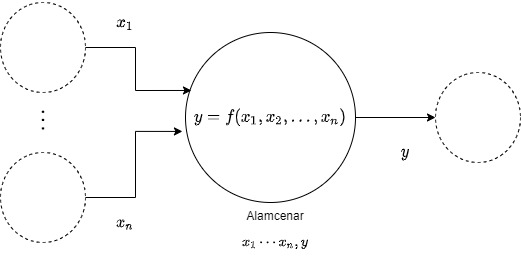
\includegraphics[scale=0.4]{im10}

\end{center}

\end{frame}

%%%%%%%%%%%%%%%%%%%%%%%%%%%%%%%%%%%%%%%%%%%%%%%%%%%%%%%%%%%%%%%%%%%%%%%%%%%%%%%%%%%%%%%%%%%%%%%%%%%%%%%%%%%%%
\begin{frame}
\frametitle{Gráficas para datos}
Ejercicio 2. Una bolsa de tamaño botana de dulces de cacahuate M\&M’s contiene 21 dulces con los colores que se indican en la tabla. La variable “color” es cualitativa. Encuentre la frecuencia, frecuencia relativa y porcentaje. Realice una grafica de barras ordenadas de mayor a menor (gráfica de Pareto).
\begin{center}
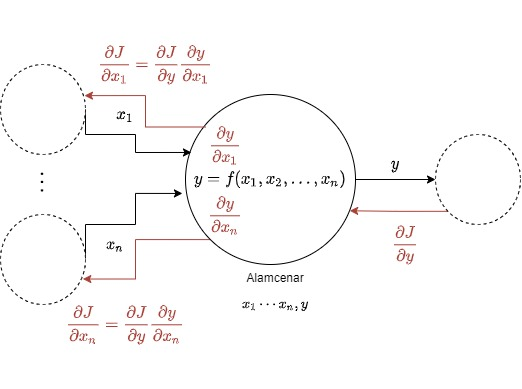
\includegraphics[scale=0.4]{im11}
\end{center}

\end{frame}
%%%%%%%%%%%%%%%%%%%%%%%%%%%%%%%%%%%%%%%%%%%%%%%%%%%%%%%%%%%%%%%%%%%%%%%%%%%%%%%%%%%%%%%%%%%%%%%%%%%%%%%%%%%%%
\begin{frame}
\frametitle{Gráficas de líneas}
Cuando una variable cuantitativa se registra en el tiempo a intervalos igualmente espaciados (por ejemplo diario, semanal, mensual, trimestral o anual), el conjunto de datos forma una serie de tiempo. Los datos de una serie de tiempo se presentan con más efectividad en una gráfica de líneas con el tiempo como eje horizontal.
\end{frame}
%%%%%%%%%%%%%%%%%%%%%%%%%%%%%%%%%%%%%%%%%%%%%%%%%%%%%%%%%%%%%%%%%%%%%%%%%%%%%%%%%%%%%%%%%%%%%%%%%%%%%%%%%%%%%
\begin{frame}
\frametitle{Gráficas de líneas}
\begin{center}
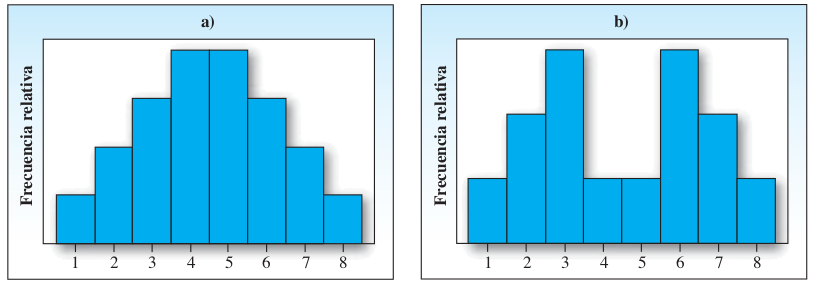
\includegraphics[scale=0.5]{im12}
\end{center}
\begin{center}
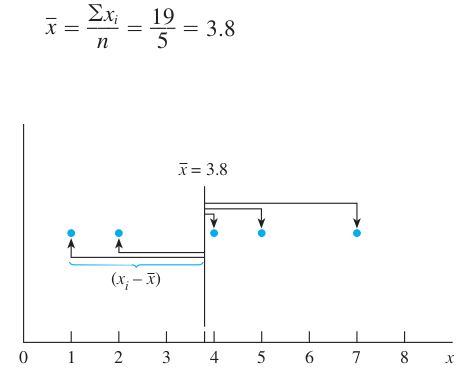
\includegraphics[scale=0.5]{im13}
\end{center}
\end{frame}
%%%%%%%%%%%%%%%%%%%%%%%%%%%%%%%%%%%%%%%%%%%%%%%%%%%%%%%%%%%%%%%%%%%%%%%%%%%%%%%%%%%%%%%%%%%%%%%%%%%%%%%%%%%%%
\begin{frame}
\frametitle{Gráficas de puntos}
La gráfica más sencilla para datos cuantitativos es la gráfica de puntos. Para un conjunto pequeño de mediciones. 
\begin{center}
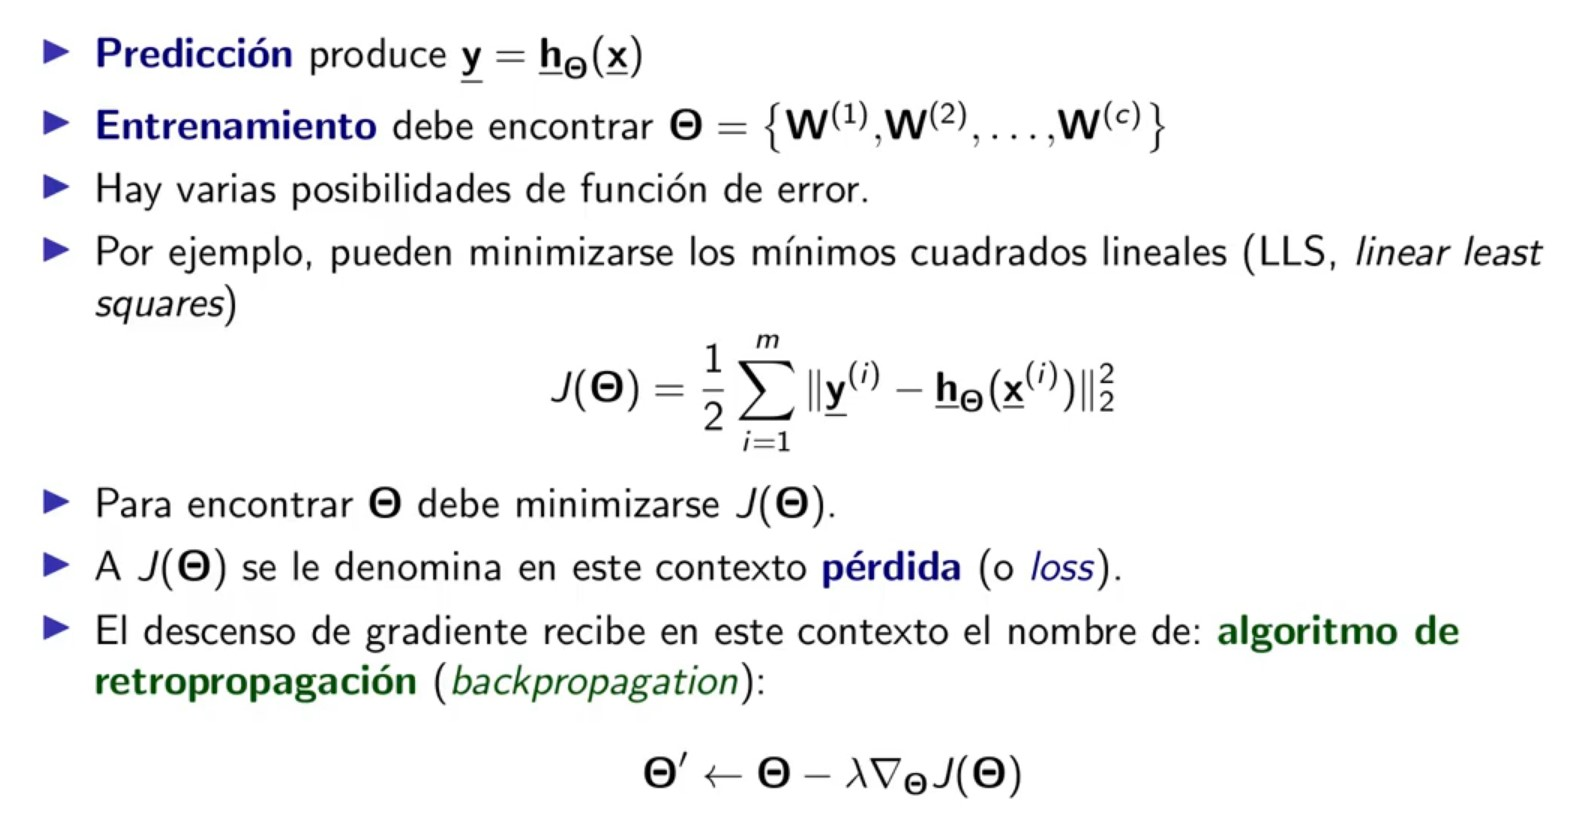
\includegraphics[scale=0.35]{im14}
\end{center}
\end{frame}
%%%%%%%%%%%%%%%%%%%%%%%%%%%%%%%%%%%%%%%%%%%%%%%%%%%%%%%%%%%%%%%%%%%%%%%%%%%%%%%%%%%%%%%%%%%%%%%%%%%%%%%%%%%%%
\begin{frame}
\frametitle{Gráficas de tallo y hoja}
Otra forma sencilla de exhibir la distribución de un conjunto de datos cuantitativos es la gráfica de tallo y hoja. Esta gráfica presenta una exhibición gráfica de los datos usando los valores numéricos reales de cada punto de datos.

\begin{center}
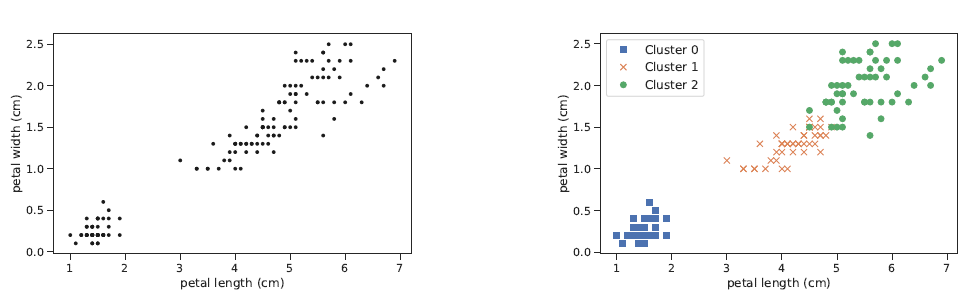
\includegraphics[scale=0.5]{im15}
\end{center}
\end{frame}
%%%%%%%%%%%%%%%%%%%%%%%%%%%%%%%%%%%%%%%%%%%%%%%%%%%%%%%%%%%%%%%%%%%%%%%%%%%%%%%%%%%%%%%%%%%%%%%%%%%%%%%%%%%%%
\begin{frame}
\frametitle{Gráficas de tallo y hoja}
Para crear el tallo y hoja, se puede dividir cada observación entre las unidades y las decenas. El número a la izquierda es el tallo; el de la derecha es la hoja.

\begin{center}
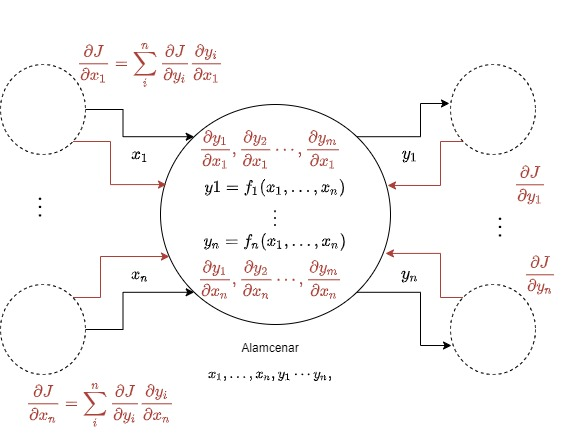
\includegraphics[scale=0.5]{im16}
\end{center}
\end{frame}
%%%%%%%%%%%%%%%%%%%%%%%%%%%%%%%%%%%%%%%%%%%%%%%%%%%%%%%%%%%%%%%%%%%%%%%%%%%%%%%%%%%%%%%%%%%%%%%%%%%%%%%%%%%%%
\begin{frame}
\frametitle{Gráficas de tallo y hoja}
A veces las opciones de tallo disponibles resultan en una gráfica que contiene muy pocos tallos y un gran número de hojas dentro de cada tallo. En esta situación, se pueden
prolongar los tallos al dividir cada uno en varias líneas, dependiendo de los valores de hojas que se les asignen.

\begin{center}
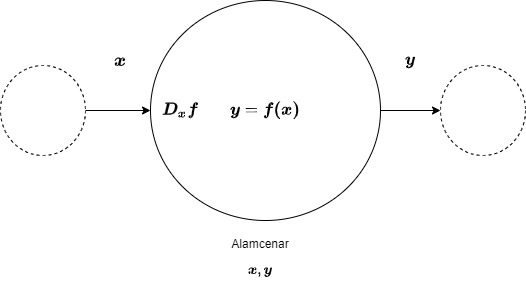
\includegraphics[scale=0.5]{im17}
\end{center}
\end{frame}
%%%%%%%%%%%%%%%%%%%%%%%%%%%%%%%%%%%%%%%%%%%%%%%%%%%%%%%%%%%%%%%%%%%%%%%%%%%%%%%%%%%%%%%%%%%%%%%%%%%%%%%%%%%%%
\begin{frame}
\frametitle{Gráficas de tallo y hoja}

\begin{center}
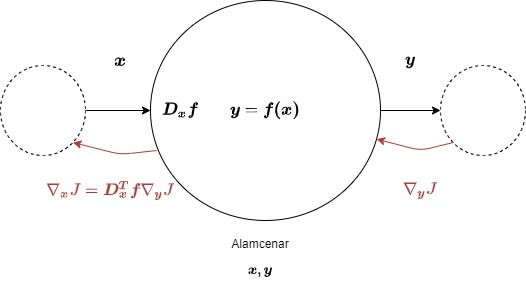
\includegraphics[scale=0.5]{im18}
\end{center}
\end{frame}
%%%%%%%%%%%%%%%%%%%%%%%%%%%%%%%%%%%%%%%%%%%%%%%%%%%%%%%%%%%%%%%%%%%%%%%%%%%%%%%%%%%%%%%%%%%%%%%%%%%%%%%%%%%%%
\begin{frame}
\frametitle{Histograma}
Un histograma de frecuencia relativa, para un conjunto de datos cuantitativo es una gráfica de barras en la que la altura de la barra muestra “con qué frecuencia” (medida como proporción o frecuencia relativa) las mediciones caen en una clase o subintervalo particular. Las clases o subintervalos se grafican a lo largo del eje horizontal.
\end{frame}
%%%%%%%%%%%%%%%%%%%%%%%%%%%%%%%%%%%%%%%%%%%%%%%%%%%%%%%%%%%%%%%%%%%%%%%%%%%%%%%%%%%%%%%%%%%%%%%%%%%%%%%%%%%%%
\begin{frame}
\frametitle{Histograma}
\begin{center}
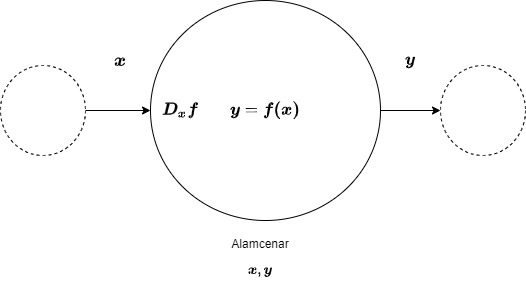
\includegraphics[scale=0.5]{im17}
\end{center}
\end{frame}
%%%%%%%%%%%%%%%%%%%%%%%%%%%%%%%%%%%%%%%%%%%%%%%%%%%%%%%%%%%%%%%%%%%%%%%%%%%%%%%%%%%%%%%%%%%%%%%%%%%%%%%%%%%%%
\begin{frame}
\frametitle{Histograma}
\begin{center}
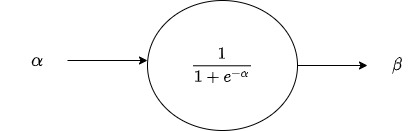
\includegraphics[scale=0.5]{im19}
\end{center}
\end{frame}
%%%%%%%%%%%%%%%%%%%%%%%%%%%%%%%%%%%%%%%%%%%%%%%%%%%%%%%%%%%%%%%%%%%%%%%%%%%%%%%%%%%%%%%%%%%%%%%%%%%%%%%%%%%%%
\begin{frame}
\frametitle{Histograma}
\begin{center}
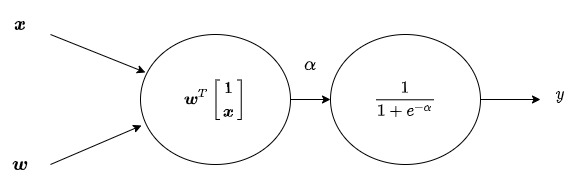
\includegraphics[scale=0.5]{im20}
\end{center}
\end{frame}
%%%%%%%%%%%%%%%%%%%%%%%%%%%%%%%%%%%%%%%%%%%%%%%%%%%%%%%%%%%%%%%%%%%%%%%%%%%%%%%%%%%%%%%%%%%%%%%%%%%%%%%%%%%%%
\begin{frame}
\frametitle{Ejercicios}
Preescolar A continuación se dan las
edades (en meses) a los que se inscribieron por
primera vez 50 niños en una escuela preescolar.
\begin{center}
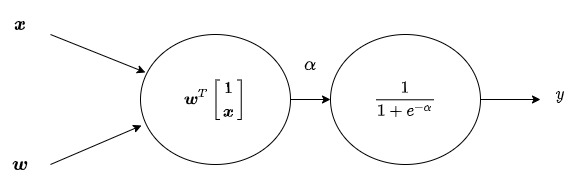
\includegraphics[scale=0.5]{im20}
\end{center}
\end{frame}
%%%%%%%%%%%%%%%%%%%%%%%%%%%%%%%%%%%%%%%%%%%%%%%%%%%%%%%%%%%%%%%%%%%%%%%%%%%%%%%%%%%%%%%%%%%%%%%%%%%%%%%%%%%%%
\begin{frame}
\frametitle{Histograma}
a. Construya una gráfica de tallo y hoja para los datos.

b. Construya un histograma de frecuencia relativa para
estos datos. Empiece en la frontera inferior de la
primera clase en 30 y use un ancho de clase de 5 meses.

c. Compare las gráficas de los incisos a) y b). ¿Hay
alguna diferencia importante que le haría escoger una
como el mejor método para exhibir los datos?
\end{frame}
%%%%%%%%%%%%%%%%%%%%%%%%%%%%%%%%%%%%%%%%%%%%%%%%%%%%%%%%%%%%%%%%%%%%%%%%%%%%%%%%%%%%%%%%%%%%%%%%%%%%%%%%%%%%%
\begin{frame}
\frametitle{Histograma}
d. ¿Qué proporción de los niños tenían 35 meses
(2 años, 11 meses) o más, pero menos de 45 meses
(3 años, 9 meses) de edad cuando se inscribieron
por primera vez en preescolar?

e. Si un niño fuera seleccionado al azar de este grupo de
niños, ¿cuál es la probabilidad de que tuviera menos
de 50 meses de edad (4 años, 2 meses) cuando se
inscribió por primera vez en preescolar?
\end{frame}
%%%%%%%%%%%%%%%%%%%%%%%%%%%%%%%%%%%%%%%%%%%%%%%%%%%%%%%%%%%%%%%%%%%%%%%%%%%%%%%%%%%%%%%%%%%%%%%%%%%%%%%%%%%%%
\end {document}



                                                  






